\scanpage{15}
\figure{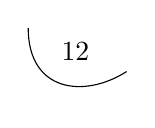
\begin{tikzpicture}[x=1cm,y=1cm]
\node at (0,0) {\mspage{12}};
\draw (-.6,.3) .. controls (-.6,-.5) and (.1,-.6) .. (.65,-.25);
\end{tikzpicture}}
\deleted{\unsure{Thus the}} $\Phi_0$ is a free module over $\mathbb Z$, generated by the
\[
\varphi_i^{\beta,\alpha}\quad\deleted{\unsure{\pi_{i\alpha}}}\qquad 0\leq i\leq n,\quad0\leq\alpha,\beta\leq2n-i
\]
\deleted{\[
\left\{\quad L^j\pi_{i,\alpha}\quad\varphi_{i,\alpha}^{j,\beta}\quad\unsure{\pi_{i\alpha}}\quad\text{for}\quad
\left\{\begin{aligned}
\unsure{i,j}\quad0\leq i\leq2n,\ 0\leq j\leq2n,\ \alpha,\beta\geq0\\
i-2\alpha=j-2\beta\geq0\\
\unsure{i<j}
\end{aligned}\right.\right.
\]}
\margin{$\mathbb Z$ can be replaced by any ring}
\deleted{$\varphi_{i,\alpha}^{j,\beta}$ is zero on the components}
defined by
\inserted{\[
\left|\begin{aligned}
\varphi_i^{\beta\alpha}&=L_0^{\beta-\alpha}\pi_{i+2\alpha,\alpha}\quad\text{if }\alpha\leq\beta\\
\varphi_i^{\beta\alpha}&=\Lambda_0^{\alpha-\beta}\pi_{i+2\alpha,\alpha}\quad\text{if }\alpha\geq\beta
\end{aligned}\right.
\]}
\deleted{\[
\left\{\begin{aligned}
\varphi_{i,\alpha}^{j,\beta}&=L_0^{\beta-\alpha}\pi_{i,\alpha}=\pi_{j,\beta}L_0^{\beta-\alpha}\quad\text{if }\alpha\leq\beta\\
\varphi_{i,\alpha}^{j,\beta}&=\Lambda_0^{\alpha-\beta}\pi_{i,\alpha}=\pi_{j,\beta}\Lambda_0^{\alpha-\beta}\quad\text{if }\alpha\geq\beta
\end{aligned}\right.
\]}
i.e. we have a basis consisting of the
\deleted{\[
\left\{L^\beta\pi_{i,\alpha}\quad\left\{\begin{aligned}
0\leq i\leq2n,\quad\alpha\geq0\quad\text{thus }i-2\alpha\geq0\\
0\leq2\alpha\leq i\\
0\leq\beta
\end{aligned}\right.\right.
\]}
\margin{\[
\begin{gathered}
\varphi_{i'}^{\beta',\alpha'}\varphi_i^{\beta,\alpha}\\
\deleted{\unsure{\varphi_{i,\alpha}^{j,\beta}\varphi_{i',\alpha'}^{j',\beta'}}}
\end{gathered}
=\left|\begin{array}{ll}
0&\text{if }\deleted{\unsure{i-2\alpha\neq j-2\beta}}\inserted{i\neq i'\text{ or }\beta\neq\alpha'}\\
\varphi_i^{\beta',\alpha}\deleted{\unsure{\alpha'}}&\text{otherwise}
\end{array}\right.
\]}
\margin{\figure{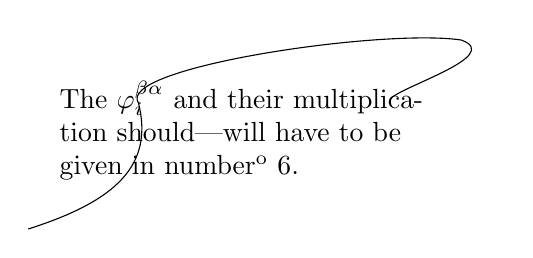
\begin{tikzpicture}
\node[align=left,text width=4.8cm,inner sep=8pt] (a) at (0,0) {The $\varphi_i^{\beta\alpha}$ and their multiplication \unsure{should|will have to} be given in number\textsuperscript{o} 6.};
\draw (-2.8,-1.25) .. controls (-1.7,-.9) and (-1.2,-.45) .. (-1.4,.35) .. controls (-1.7,.8) and (1.7,1.3) .. (2.7,1.15) .. controls (3.25,.95) and (1.9,.55) .. (1.8,.4);
\end{tikzpicture}}}

The multiplication of the elements of this basis of course does not depend on the choice of $\mathbf M_0,\xi_0$ (nor on the fact that we are over the ring $\mathbb Z$ ....), so the ring $\Phi_0$ is indeed determined in terms of the \inserted{\figure{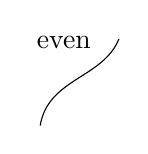
\begin{tikzpicture}[x=1cm,y=1cm]
\node at (0,.35) {even};
\draw (-.3,-.7) .. controls (-.2,-.1) and (.5,-.1) .. (.7,.4);
\end{tikzpicture}}} integer $2n$.

\uline{Proposition} Returning to the datum of $M^*$ as in number\textsuperscript{o} 1, and of $\mathcal E$ a graded sub-\deleted{algebra}\inserted{ring} of \deleted{$\unsure{\mathcal E}$} $\operatorname{End}(M^*)$.
\inserted{Let $L\in\mathcal E^{(2)}$}
Equivalent conditions

(i) The endomorphism $L$ of $M^*$ satisfies the \deleted{Hard} Lefschetz condition and the associated operator $\Lambda$ is in $\mathcal E$.
(that is to say we are in the conditions of the theorem of number\textsuperscript{o} 6).

(ii) There exists a homomorphism of graded rings
\[
\varphi:\Phi_0\longrightarrow\mathcal E
\]
\mspage{14}
